\subsection{CONSUMIDORES DIRECTOS}

Se consideran consumidores directos a los administradores o due�os de estacionamiento. De acuerdo a una investigaci�n realizada por la UNAM. En el DF hay 1,783 estacionamientos p�blicos, con m�s de 300 mil cajones \cite{publimetro}. La Figura \ref{fig:graficaEstacionamientosPorArea} muestras las 6 delegaciones (m�s de 84\% del total) con mayor n�mero de estacionamiento, asi como, el porcentaje que le corresponde.

\begin{figure}[ht]
	\centering
	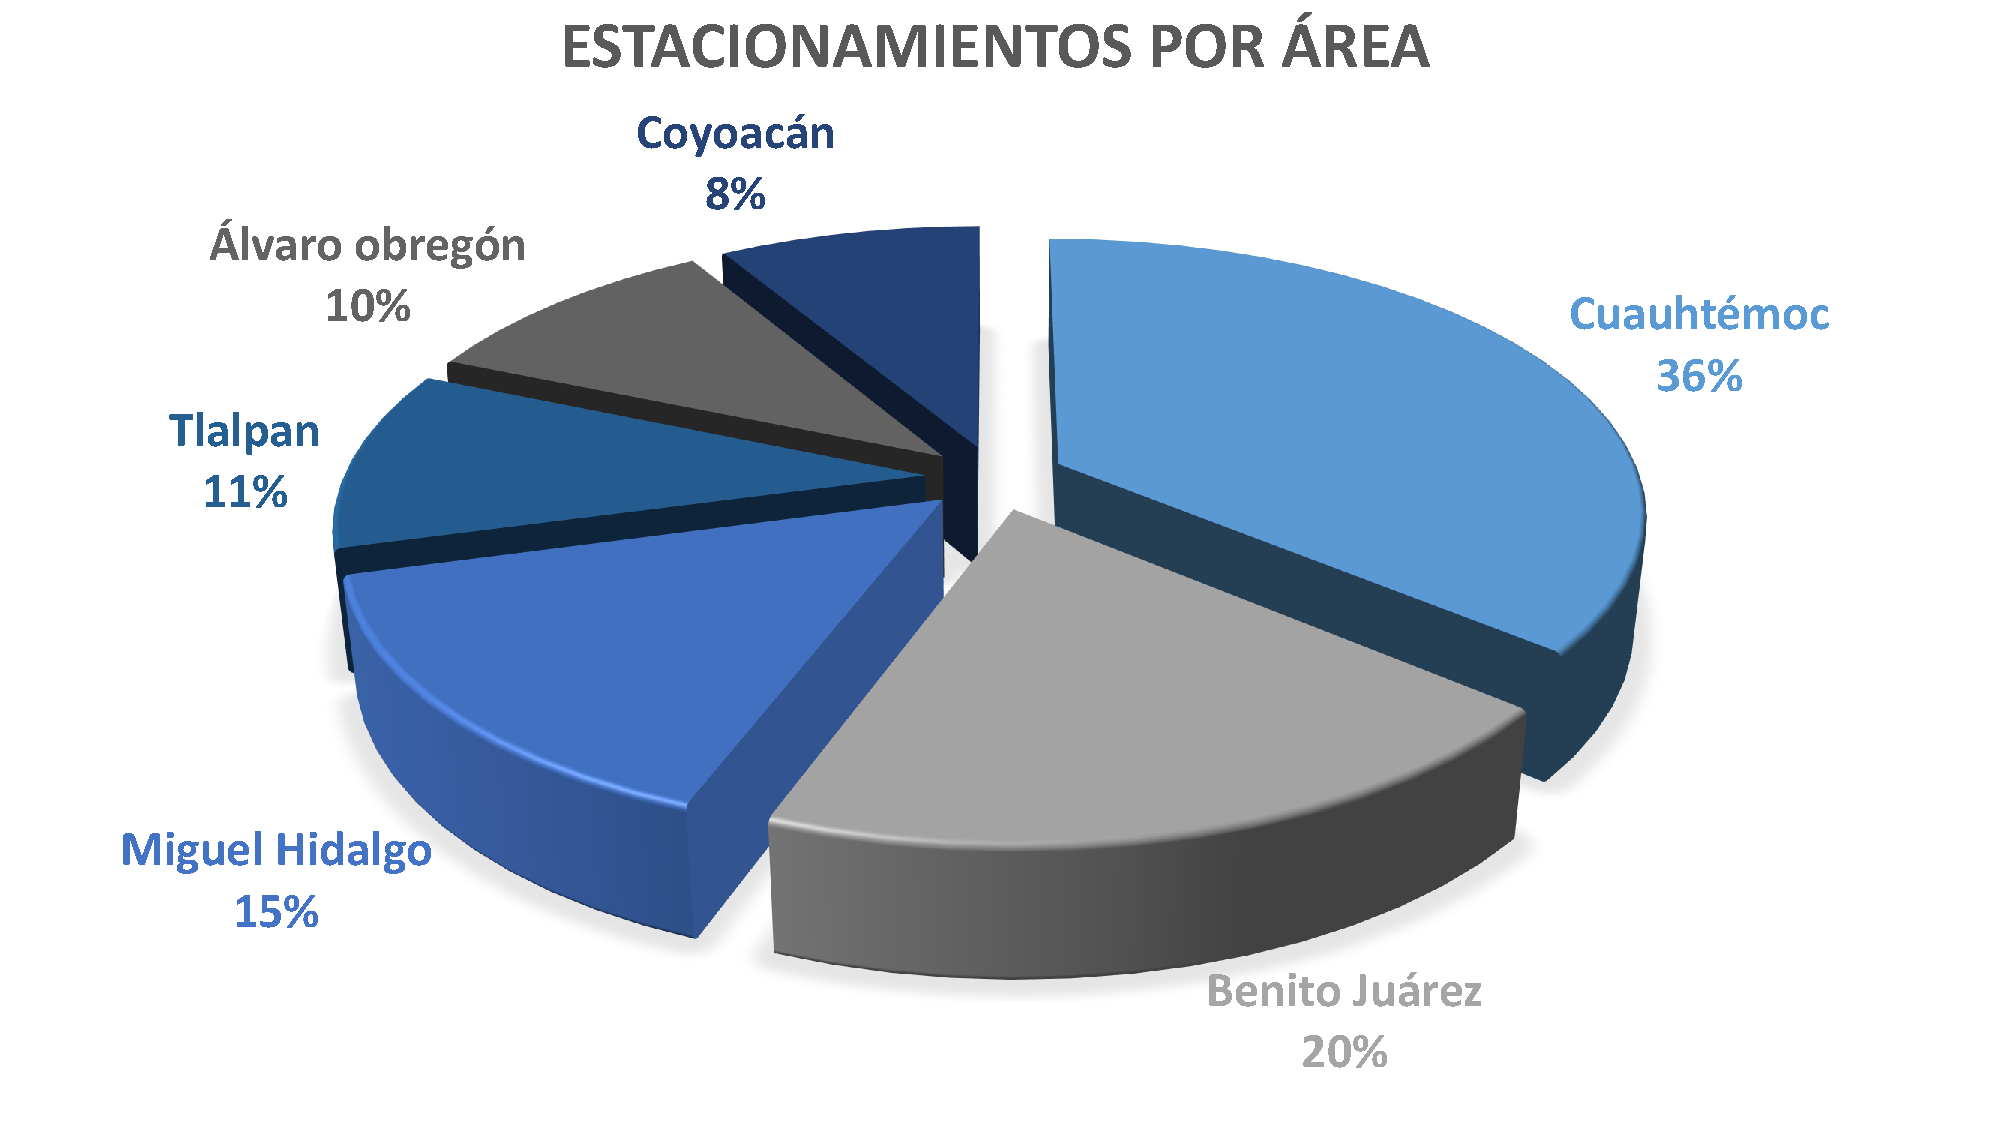
\includegraphics[scale=.3]{./analisisDeLaDemanda/source/estacionamientosPorArea}
	\caption{Estacionamientos por �rea en el DF}
	\label{fig:graficaEstacionamientosPorArea}
\end{figure}


Otra opci�n para estacionar en veh�culo es el parqu�metro, datos obtenidos a trav�s de ecoParq \cite{ecoparq}, hay 1,229 parqu�metros instalados, atendiendo a 19,890 cajones en la v�a publica, distribuidos de la como se muestra en el Cuadro \ref{tab:Parquimetros}.

\begin{table}[h]
	\centering
	\begin{tabular}{|l|c|c|}
		\hline COLONIA & PARQUIMETRO & CAJONES \\ 
		\hline Anzures & 113 & 1695 \\ 
		\hline Lomas-Virreyes & 162 & 3250 \\ 
		\hline Nochebuena & 32 & 500 \\ 
		\hline Polanco & 416 & 6240 \\ 
		\hline Roma/Condesa & 353 & 5535 \\ 
		\hline Florencia & 85 & 1470 \\ 
		\hline Ciudad de los deportes & 40 & 760 \\ 
		\hline Cr�dito - Constructor & 28 & 440 \\ 
		\hline
	\end{tabular}
	\label{tab:Parquimetros}
	\caption{Parquimetros y cajones por Colonia.}
\end{table}


Tomando como ejemplo la delegaci�n Cuauht�moc s�lo el 12\% de los autom�viles utilizan los aparcamientos p�blicos, mientras que 57\% aloja su veh�culo en estacionamientos privados, otro 28\% se estaciona en la v�a p�blica y s�lo 3\% de la poblaci�n lo hace en garaje propio \cite{autobild}.

\begin{figure}[h]
	\centering
	\includegraphics[scale=.3]{./analisisDeLaDemanda/source/TiposDeAlojamiento}
	\caption{Tipos de alojamiento, Delegacion Cuauht�moc}
	\label{fig:tiposDeAlojamiento}
\end{figure}


\subsection{CONSUMIDORES INDIRECTOS}
Consideramos a los consumidores indirecots como los usuarios que har�n uso del estacionamiento(usuarios finales). Seg�n datos del INEGI la flota  vehicular  registrada  en  el M�xico Distrito Federal se estima en 36.7 millones de veh�culos. \cite{INEGI}. En la Figura \ref{fig:vehiculosPorAno} podemos observar la cantidad de veh�culos y su tipo, asi como, el crecimiento que han tenido a�o con a�o desde 2003. 

\begin{figure}[h]
	\centering
	\includegraphics[scale=.5]{./analisisDeLaDemanda/source/VehiculosPorAno}
	\caption{N�mero de veh�culos por a�o seg�n su clase. Cifra mostrada en cientos de miles}
	\label{fig:vehiculosPorAno}
\end{figure}

El tipo de demanda que se detecta es insatisfecha, ya que, la gran mayor�a  de los estacionamientos (peque�os y medianos) opera solo con un dispositivo \textit{checador} que utilizan para contar el tiempo dentro del estacionamiento, y un registro  donde llevan el control de pensionados, y el total de las entradas. Figura \ref{fig:EstacionamientoChicoCompleto}.
\\
\begin{figure}
	\centering
  	\subfloat[Estacionamiento]{
   		\label{fig:Estacionamiento}
    	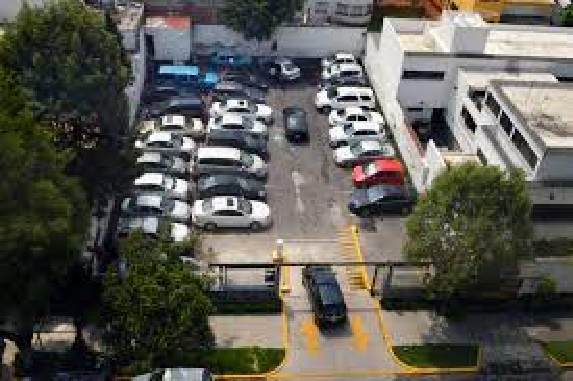
\includegraphics[width=0.3\textwidth]{./analisisDeLaDemanda/source/estacionamientoPequeno.pdf}
    }
  	\subfloat[Checador]{
   		\label{fig:relojChecador}
    	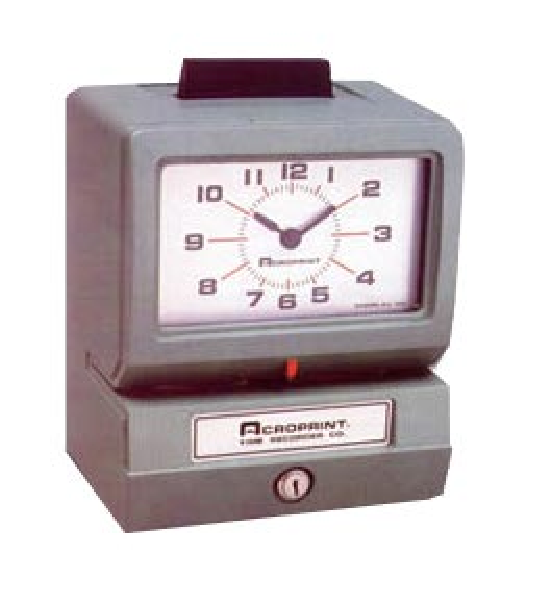
\includegraphics[width=0.15\textwidth]{./analisisDeLaDemanda/source/relojChecador.pdf}
    }
  	\subfloat[Conejo]{
   		\label{fig:libreta}
    	
\includegraphics[width=0.15\textwidth]{./analisisDeLaDemanda/source/libreta.pdf}
    }
 	\caption{Estacionamiento chico y principales componentes}
 	\label{fig:EstacionamientoChicoCompleto}
\end{figure}

%SAE se enfoca en los estacionamientos peque�os y medianos ya que ellos representan un gran segmento del mercado y %resulta muy favorable para el ellos el uso de SAE (GANAR-GANAR).

Existen otro tipo de estacionamientos, estos los podemos encontrar en centros comerciales, plazas, s�per mercados, cines, teatros, zonas, hospitales, etc. Estos estacionamientos los definimos con \textit{estacionamientos grandes}. Estos tienen la caracter�stica de tener mayores ingresos y por ende poseen una mejor infraestructura. Figura \ref{fig:EstacionamientoGrandeCompleto}. Usualmente son administrador por un tercero y tiene sistema que automatiza las tareas operativas.  La desventaja principal de este tipo de estacionamientos es que el due�o del estacionamiento pierde el control del mismo y sus ingresos son   reducidos en gran medida, hasta de un 50\% de total, siempre y cuando el tercero haya recuperada la inversi�n inicial echa.  
Este tipo de estacionamientos no es nuestro principal cliente, pues ya posee un grado de automatizaci�n mayor; sin embargo SAE API brinda un conjunto de m�todos que pueden utilizar los sistemas externos para hacer uso de la plataforma que brinda SAE y con ellos aprovechar las ventajas que este brinda.


\begin{figure}
	\centering
  	\subfloat[modulodeCobro]{
   		\label{fig:EstacionamientoGrande}
    	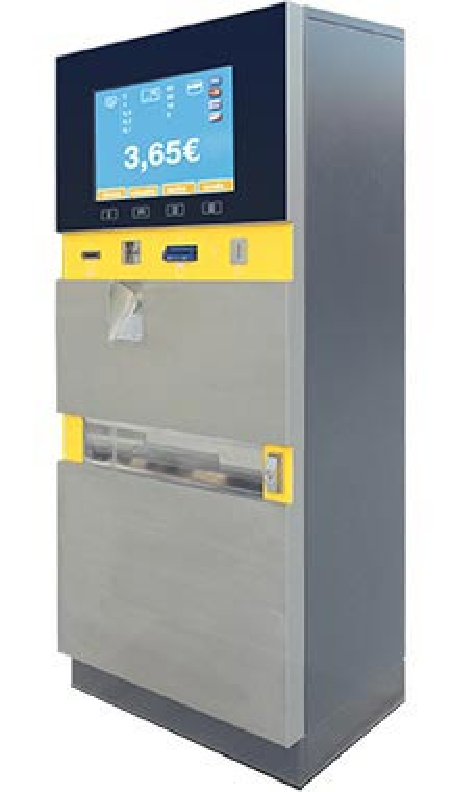
\includegraphics[width=0.23\textwidth]{./analisisDeLaDemanda/source/mouloDeCobro.pdf}
    }
  	\subfloat[pluma]{
   		\label{fig:pluma}
    	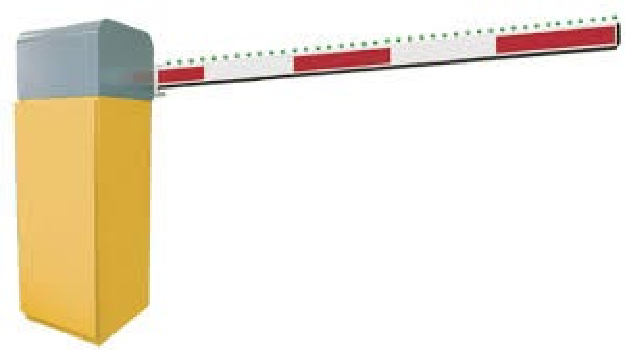
\includegraphics[width=0.5\textwidth]{./analisisDeLaDemanda/source/pluma.pdf}
    }
  	\subfloat[boletera]{
   		\label{fig:boletera}
    	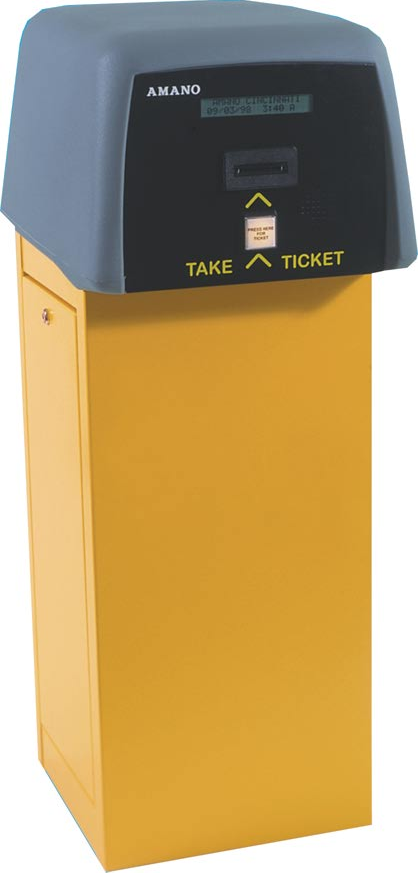
\includegraphics[width=0.14\textwidth]{./analisisDeLaDemanda/source/boletera.pdf}
    }
 	\caption{Infraestructura de estacionamientos grandes}
 	\label{fig:EstacionamientoGrandeCompleto}
\end{figure}

\newpage

